\documentclass[10pt]{article}

\usepackage[a4paper,top=18mm,bottom=18mm,left=19mm,right=19mm,headsep=7mm]{geometry}
\usepackage[T1]{fontenc}
\usepackage{newtxtext,newtxmath}
\usepackage{microtype}
\usepackage[table]{xcolor}
\usepackage{booktabs}
\usepackage{tabularx}
\usepackage{array}
\usepackage{graphicx}
\usepackage{amsmath}
\usepackage{caption}
\usepackage{fancyhdr}
\usepackage{titlesec}
\usepackage{enumitem}
\usepackage[hidelinks]{hyperref}

\definecolor{IEEEBlue}{HTML}{163A59}
\definecolor{RuleGray}{HTML}{9AA7B1}
\definecolor{TableHead}{HTML}{EAF0F4}
\definecolor{SoftGray}{HTML}{F5F7F8}

\setlength{\parindent}{1.25em}
\setlength{\parskip}{0.2em}
\setlength{\tabcolsep}{5pt}
\setlength{\headheight}{19pt}
\renewcommand{\arraystretch}{1.08}
\raggedbottom

\pagestyle{fancy}
\fancyhf{}
\fancyhead[L]{\footnotesize\color{IEEEBlue}\textsc{Supplementary Material}}
\fancyhead[R]{\footnotesize\color{RuleGray}Trace-Aware Power System Scheduling}
\fancyfoot[C]{\footnotesize\thepage}
\renewcommand{\headrulewidth}{0.4pt}
\renewcommand{\headrule}{\hbox to\headwidth{\color{RuleGray}\leaders\hrule height \headrulewidth\hfill}}

\titleformat{\section}
  {\large\bfseries\color{IEEEBlue}}
  {\thesection}{0.65em}{}
  [\vspace{-0.35em}\color{RuleGray}\titlerule]
\titlespacing*{\section}{0pt}{1.15em}{0.65em}

\captionsetup{
  font=small,
  labelfont={bf,color=IEEEBlue},
  textfont=small,
  justification=centering,
  hypcap=false,
  skip=5pt
}

\renewcommand{\thesection}{S\arabic{section}}
\renewcommand{\thetable}{S\arabic{table}}
\renewcommand{\thefigure}{S\arabic{figure}}
\renewcommand{\theequation}{S\arabic{equation}}

\newcolumntype{Y}{>{\raggedright\arraybackslash}X}
\newcolumntype{C}{>{\centering\arraybackslash}X}
\newcommand{\tableheader}{\rowcolor{TableHead}}

\begin{document}

\begin{center}
  {\small\bfseries\color{IEEEBlue}\MakeUppercase{Supplementary Material}}\\[0.55em]
  {\LARGE\bfseries Trace-Aware Power System Scheduling with\\[0.18em]
  Heterogeneous Power Sources: A Learning-Based Framework}\\[0.8em]
  {\normalsize Kai Xiong, Xiaomeng Ai, Jingguan Liu, Shichang Cui, Jiakun Fang,\\
  Junliang Ye, Xiaohu Ge, and Jinyu Wen}\\[0.35em]
  {\small State Key Laboratory of Advanced Electromagnetic Technology,\\
  Huazhong University of Science and Technology, Wuhan, China}\\[0.2em]
  {\small Corresponding author: Xiaomeng Ai (\href{mailto:xiaomengai@hust.edu.cn}{xiaomengai@hust.edu.cn})}
\end{center}

\vspace{0.3em}
\noindent\colorbox{SoftGray}{%
  \parbox{\dimexpr\textwidth-2\fboxsep\relax}{\small
  This document accompanies the paper cited above. It provides the test-system settings,
  neural-network training and MILP reformulation details, and supplementary figures used to
  support the numerical studies.}}

\section{Modified IEEE 14-Bus Test System}

The small-system study is based on the MATPOWER \texttt{case14} data, with branch 4--5
removed. The wind source, scheduling settings, and source-share requirement are introduced
as summarized below.

\begin{minipage}[t]{0.455\textwidth}
\captionsetup{type=table}
\captionof{table}{Principal system and scheduling settings.}
\label{tab:case14_summary}
\footnotesize
\begin{tabularx}{\linewidth}{@{}Y>{\raggedleft\arraybackslash}p{0.42\linewidth}@{}}
\toprule
\tableheader Parameter & Value \\
\midrule
Base power & 100 MVA \\
Buses / branches & 14 / 19 \\
Thermal units & 5 \\
Thermal-unit buses & 1, 2, 3, 6, 8 \\
Wind farm & 100 MW at Bus 3 \\
Requirement bus & Bus 4 \\
Horizon / interval & 24 h / 1 h \\
Minimum output & $0.2P^{\max}$ \\
Ramp-up/down limits & $0.6P^{\max}$/h \\
Minimum up/down time & 3 h / 3 h \\
Startup cost & \$3000/start \\
Cost approximation & Four segments \\
\bottomrule
\end{tabularx}
\end{minipage}
\hfill
\begin{minipage}[t]{0.50\textwidth}
\captionsetup{type=table}
\captionof{table}{Thermal-unit parameters.}
\label{tab:case14_gen}
\footnotesize
\setlength{\tabcolsep}{3.6pt}
\begin{tabular}{@{}ccccccc@{}}
\toprule
\tableheader Unit & Bus & \multicolumn{2}{c}{$P$ (MW)} & $c_2$ & $c_1$ & $c_0$ \\
\cmidrule(lr){3-4}
 & & $P^{\max}$ & $P^{\min}$ & & & \\
\midrule
TU1 & 1 & 332.4 & 66.48 & 0.0430 & 19 & 0 \\
TU2 & 2 & 140.0 & 28.00 & 0.2500 & 20 & 0 \\
TU3 & 3 & 100.0 & 20.00 & 0.0100 & 40 & 0 \\
TU4 & 6 & 100.0 & 20.00 & 0.0100 & 41 & 0 \\
TU5 & 8 & 100.0 & 20.00 & 0.0100 & 42 & 0 \\
\bottomrule
\end{tabular}

\vspace{0.75em}
\captionsetup{type=table}
\captionof{table}{Neural-network settings.}
\label{tab:case14_nn}
\footnotesize
\begin{tabularx}{\linewidth}{@{}Y>{\raggedleft\arraybackslash}p{0.52\linewidth}@{}}
\toprule
\tableheader Parameter & Value \\
\midrule
Retained samples & 34,427 \\
Train / validation / test & 70\% / 15\% / 15\% \\
Inputs & Total wind; TU1--TU5 outputs \\
Outputs & Shares at Buses 3 and 4 \\
Hidden layers & [24, 12] \\
Activation & ReLU \\
\bottomrule
\end{tabularx}
\end{minipage}

\vspace{0.8em}
The base active-load vector is
\begin{equation}
P^{\mathrm{L}}_{\mathrm{base}}=
[0,21.7,94.2,47.8,7.6,11.2,0,0,29.5,9.0,3.5,6.1,13.5,14.9]\ \mathrm{MW}.
\label{eq:base_load}
\end{equation}
Table~\ref{tab:profiles} gives the hourly factors used in the 24-h scheduling study.

\begin{table}[!ht]
\centering
\caption{Hourly load and wind factors.}
\label{tab:profiles}
\small
\setlength{\tabcolsep}{8pt}
\begin{tabular}{@{}ccc@{\hspace{1.5cm}}ccc@{}}
\toprule
\tableheader Hour & Load & Wind & Hour & Load & Wind \\
\midrule
 1 & 0.7389 & 0.6602 & 13 & 0.8923 & 0.6053 \\
 2 & 0.7187 & 0.6830 & 14 & 0.8877 & 0.6038 \\
 3 & 0.7035 & 0.7083 & 15 & 0.8840 & 0.6068 \\
 4 & 0.6983 & 0.6925 & 16 & 0.8849 & 0.9050 \\
 5 & 0.7040 & 0.6845 & 17 & 0.8941 & 0.8218 \\
 6 & 0.7251 & 0.7142 & 18 & 0.9345 & 0.8220 \\
 7 & 0.7764 & 0.7235 & 19 & 0.9899 & 0.6870 \\
 8 & 0.8461 & 0.5415 & 20 & 0.9841 & 0.6559 \\
 9 & 0.8951 & 0.7793 & 21 & 0.9691 & 0.6720 \\
10 & 0.9094 & 0.7860 & 22 & 0.9436 & 0.6934 \\
11 & 0.9078 & 0.7215 & 23 & 0.9094 & 0.7058 \\
12 & 0.9071 & 0.6585 & 24 & 0.8674 & 0.6964 \\
\bottomrule
\end{tabular}
\end{table}

\clearpage
\section{Neural-Network Training and MILP Reformulation}

For sample $m$, let $\mathbf{x}^{(m)}$ and $\mathbf{T}^{\mathrm{G},(m)}$ denote the input and
tracing-label vectors. The input and output statistics are denoted by
$(\boldsymbol{\mu}_x,\boldsymbol{\sigma}_x)$ and
$(\boldsymbol{\mu}_y,\boldsymbol{\sigma}_y)$, respectively. The function $\sigma(\cdot)$ is
the ReLU activation, $\Theta$ collects the trainable weights and biases, and $\oslash$ and
$\odot$ denote elementwise division and multiplication. Training and output recovery are
written as
\begin{subequations}
\label{eq:supp_nn_training}
\begin{align}
\bar{\mathbf{x}}^{(m)}
&=(\mathbf{x}^{(m)}-\boldsymbol{\mu}_x)\oslash\boldsymbol{\sigma}_x,
&
\bar{\mathbf{y}}^{(m)}
&=(\mathbf{T}^{\mathrm{G},(m)}-\boldsymbol{\mu}_y)\oslash\boldsymbol{\sigma}_y,
\label{eq:supp_normalization}\\
\mathbf{z}^{1,(m)}
&=\sigma(\mathbf{W}^{1}\bar{\mathbf{x}}^{(m)}+\mathbf{b}^{1}),
&
\mathbf{z}^{p,(m)}
&=\sigma(\mathbf{W}^{p}\mathbf{z}^{p-1,(m)}+\mathbf{b}^{p}),\quad p=2,\ldots,L,
\label{eq:supp_hidden_layers}\\
\hat{\mathbf{y}}^{(m)}
&=\mathbf{W}^{L+1}\mathbf{z}^{L,(m)}+\mathbf{b}^{L+1},
&
\Theta
&=\{\mathbf{W}^{p},\mathbf{b}^{p}\}_{p=1}^{L+1},
\label{eq:supp_output_parameters}\\
\min_{\Theta}\;&\frac{1}{N_{\mathrm{sam}}}
\sum_{m=1}^{N_{\mathrm{sam}}}
\|\hat{\mathbf{y}}^{(m)}-\bar{\mathbf{y}}^{(m)}\|_2^2,
\label{eq:supp_training_loss}\\
\widetilde{\mathbf{T}}^{\mathrm{G},(m)}
&=\boldsymbol{\mu}_y+\boldsymbol{\sigma}_y\odot\hat{\mathbf{y}}^{(m)}.
\label{eq:supp_output_recovery}
\end{align}
\end{subequations}
In the scheduling model, the same forward mapping is evaluated period by period by replacing
the sample index $m$ with the scheduling index $t$.

For a hidden neuron with affine input $\hat z$, ReLU output $z=\max\{\hat z,0\}$, and valid
bounds $\underline h\leq\hat z\leq\bar h$, introduce a binary activation variable $a$. Its exact
mixed-integer linear representation is
\begin{subequations}
\label{eq:supp_relu_milp}
\begin{align}
z&\geq 0, & z&\geq \hat z,\label{eq:supp_relu_lower}\\
z&\leq \hat z-\underline h(1-a), &
z&\leq \bar h a,\qquad a\in\{0,1\}.\label{eq:supp_relu_upper}
\end{align}
\end{subequations}
When $a=0$, the constraints give $z=0$ and require $\hat z\leq0$; when $a=1$, they give
$z=\hat z\geq0$. Applying these constraints neuron by neuron, followed by the affine output
layer and denormalization, yields the MILP embedding used in the paper.

\section{Practical-Scale Transmission-System Case}

\begin{minipage}[t]{0.43\textwidth}
\captionsetup{type=table}
\captionof{table}{Principal practical-scale case settings.}
\label{tab:practical_summary}
\small
\begin{tabularx}{\linewidth}{@{}Y>{\raggedleft\arraybackslash}p{0.44\linewidth}@{}}
\toprule
\tableheader Parameter & Value \\
\midrule
Base power & 100 MVA \\
Buses / branches & 57 / 78 \\
Thermal units & 50 \\
Wind farms & 8 $\times$ 1500 MW \\
Wind-farm buses & 7, 13, 23, 25, 42, 47, 49, 53 \\
Total wind capacity & 12,000 MW \\
Requirement / slack bus & 55 / 38 \\
Horizon / interval & 24 h / 1 h \\
Line-rating multiplier & 3 \\
Cost approximation & Four segments \\
\bottomrule
\end{tabularx}
\end{minipage}
\hfill
\begin{minipage}[t]{0.54\textwidth}
\captionsetup{type=table}
\captionof{table}{Thermal-unit parameters by bus.}
\label{tab:practical_thermal}
\small
\setlength{\tabcolsep}{4.2pt}
\begin{tabular}{@{}rrrrrr@{}}
\toprule
\tableheader Bus & Units & $P^{\max}$ & $P^{\min}$ & RU/RD & $c_1$ \\
 & & \multicolumn{3}{c}{(MW or MW/h)} & \\
\midrule
 3 & 2 & 1200 & 240 & 720 & 38.5000 \\
 8 & 2 & 1320 & 264 & 792 & 41.5000 \\
 9 & 4 & 1200 & 240 & 720 & 20.0000 \\
11 & 6 & 4400 & 880 & 2640 & 30.9091 \\
14 & 2 & 1200 & 240 & 720 & 40.0000 \\
24 & 4 & 2020 & 404 & 1212 & 33.0693 \\
30 & 4 & 1920 & 384 & 1152 & 33.7500 \\
32 & 2 & 700 & 140 & 420 & 20.0000 \\
35 & 2 & 780 & 156 & 468 & 20.0000 \\
37 & 2 & 2000 & 400 & 1200 & 20.0000 \\
38 & 6 & 2400 & 480 & 1440 & 30.0000 \\
40 & 4 & 1900 & 380 & 1140 & 32.6316 \\
46 & 2 & 2000 & 400 & 1200 & 20.0000 \\
50 & 2 & 1200 & 240 & 720 & 40.0000 \\
54 & 2 & 1320 & 264 & 792 & 40.0000 \\
57 & 4 & 1800 & 360 & 1080 & 33.3333 \\
\bottomrule
\end{tabular}
\end{minipage}

\vspace{0.7em}
The listed capacity and ramping values are totals over the thermal units connected to each bus.
The common quadratic and constant cost coefficients are $c_2=0.01$ and $c_0=0$,
respectively. The quadratic costs are represented by the four-segment linear approximation
reported in Table~\ref{tab:practical_summary}.

\clearpage
\section{Supplementary Figures}

\noindent
\centering
\begin{minipage}[t]{0.36\textwidth}
\centering
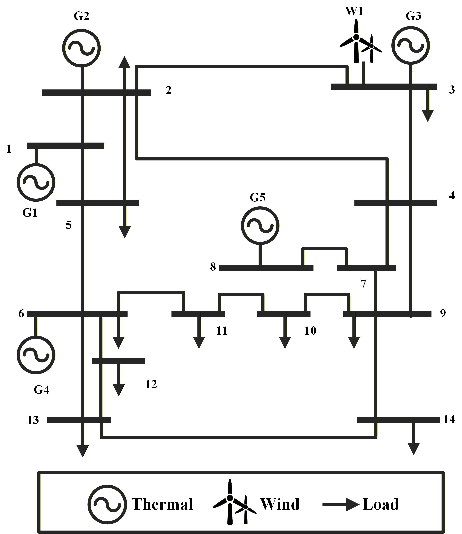
\includegraphics[width=0.96\linewidth]{figure/IEEE14-Eng.pdf}
\captionof{figure}{Topology of the modified IEEE 14-bus test system.}
\label{fig:supp_ieee14_topology}
\end{minipage}
\hfill
\begin{minipage}[t]{0.61\textwidth}
\centering
\vspace{1.0em}
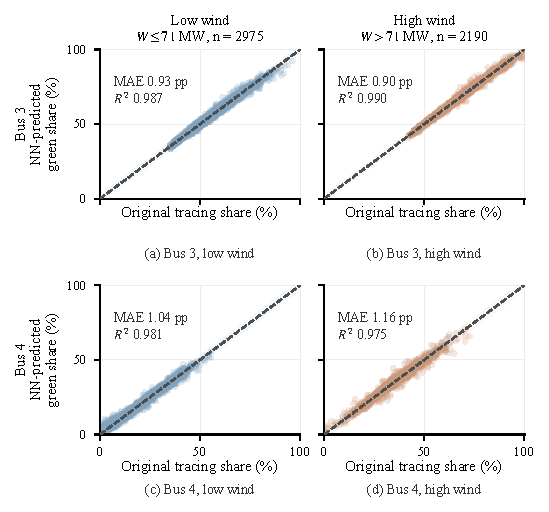
\includegraphics[width=\linewidth]{figure/ieee14_nn_generalization_regimes.pdf}
\captionof{figure}{Held-out parity comparison under low- and high-wind conditions.}
\label{fig:supp_ieee14_parity}
\end{minipage}

\end{document}
